% !TeX root = 流体力学笔记.tex
% 流体力学笔记 —— 张量代数基础
% 张量的概念、指标表示与基本运算

\section{标量、向量与张量}

之前学过的物理量分为标量和向量，其实都可以归结于张量。

表示一个物理量有很多种方式，比如\textbf{实体形式}和\textbf{分量形式}。实体形式具有\textbf{客观存在性}和\textbf{坐标无关性}；而分量形式依赖于选取的坐标系，是随着坐标变化的。

如应力：
\begin{equation}
	\boldsymbol{\sigma}=
	\begin{bmatrix}
		\sigma_{11} & \sigma_{12} & \sigma_{13} \\
		\sigma_{21} & \sigma_{22} & \sigma_{23} \\
		\sigma_{31} & \sigma_{32} & \sigma_{33}
	\end{bmatrix},
	\label{eq:应力张量表示}
\end{equation}
左侧即为实体形式，右侧为分量形式。

\section{张量的指标表示}

\subsection{向量的表示}

向量 $\boldsymbol{a}$、$\boldsymbol{b}$ 可以写成如下三种等价形式：
\begin{equation}
	\begin{aligned}
		\boldsymbol{a} & =a_{1}\boldsymbol{e}_{1}+a_{2}\boldsymbol{e}_{2}+a_{3}\boldsymbol{e}_{3}
		\;\longleftrightarrow\;
		\begin{bmatrix} a_{1} & a_{2} & a_{3} \end{bmatrix}^{\mathrm{T}}
		\;\longleftrightarrow\;
		a_{i}, \\[4pt]
		\boldsymbol{b} & =b_{1}\boldsymbol{e}_{1}+b_{2}\boldsymbol{e}_{2}+b_{3}\boldsymbol{e}_{3}
		\;\longleftrightarrow\;
		\begin{bmatrix} b_{1} & b_{2} & b_{3} \end{bmatrix}^{\mathrm{T}}
		\;\longleftrightarrow\;
		b_{j}.
	\end{aligned}
	\label{eq:向量指标表示}
\end{equation}
相应地，向量的加法与点乘可写作
\begin{equation}
	\boldsymbol{a}+\boldsymbol{b}:a_{i}+b_{i},\qquad
	\boldsymbol{a}\cdot\boldsymbol{b}=a_{i}b_{i}.
	\label{eq:向量运算指标表示}
\end{equation}

\begin{keybox}[爱因斯坦求和约定]
	这里使用\textbf{爱因斯坦求和约定}：重复下标默认求和。
\end{keybox}

向量是一阶张量。

\subsection{矩阵的表示}

二阶张量（矩阵）$\boldsymbol{C}$ 可表示为
\begin{equation}
	\boldsymbol{C}=
	\begin{bmatrix}
		c_{11} & c_{12} & c_{13} \\
		c_{21} & c_{22} & c_{23} \\
		c_{31} & c_{32} & c_{33}
	\end{bmatrix}:C_{ij}.
	\label{eq:二阶张量指标表示}
\end{equation}
即矩阵是二阶张量。

\section{张量运算}

\subsection{点乘}

\begin{equation}
	\boldsymbol{C}\cdot\boldsymbol{D}:C_{ij}D_{jk},
	\label{eq:张量点乘}
\end{equation}
结果为矩阵，即二阶张量，剩两个自由指标；
\begin{equation}
	\boldsymbol{C}\cdot\boldsymbol{x}:C_{ij}x_{j},
	\label{eq:张量与向量点乘}
\end{equation}
结果为向量，剩一个自由指标 $i$；
\begin{equation}
	\boldsymbol{y}\cdot\boldsymbol{D}\cdot\boldsymbol{x}:y_{i}D_{ij}x_{j},
	\label{eq:向量夹乘}
\end{equation}
结果为数，剩零个自由指标。

点乘的规则是：\textbf{相邻张量的相邻指标相同}。

\subsection{缩并：降两阶的手段}

\begin{equation}
	C_{ij}\Rightarrow C_{ii}.
	\label{eq:张量缩并}
\end{equation}
二阶张量缩并之后就是矩阵的迹，即二阶张量对角线元素之和，也是二阶张量特征值之和。

缩并的规则是：\textbf{张量自身一对指标相同}。

\subsection{并积}

对于两个向量
\begin{equation}
	\boldsymbol{x}\leftrightarrow x_{i},\qquad \boldsymbol{y}\leftrightarrow y_{j},
	\label{eq:并积前}
\end{equation}
其并积为
\begin{equation}
	\boldsymbol{x}\boldsymbol{y}=x_{i}y_{j}.
	\label{eq:并积}
\end{equation}

并积的规则是：\textbf{两个张量放在一起不做任何表示（指标不重复）}。

\subsection{指标表示规则}

\begin{enumerate}
	\item 每一项中，同一指标最多出现两次：
	      \begin{enumerate}
		      \item 出现一次的指标是自由指标，可以任意取值；
		      \item 出现两次的指标是哑指标，自动求和，触发爱因斯坦求和约定。
	      \end{enumerate}
	\item 指标平衡：每一项中，自由指标数相同且一一对应。
\end{enumerate}

\section{向量乘法与指标运算}

对于
\begin{equation}
	\boldsymbol{a}=a_{i}\boldsymbol{e}_{i},\qquad \boldsymbol{b}=b_{i}\boldsymbol{e}_{i},
	\label{eq:向量的基表示}
\end{equation}
有
\begin{itemize}
	\item \textbf{点乘}：$\boldsymbol{a}\cdot\boldsymbol{b}=a_{i}b_{i}$；
	\item \textbf{叉乘}：$\boldsymbol{a}\times\boldsymbol{b}=a_{i}b_{j}\varepsilon_{ijk}\boldsymbol{e}_{k}$；
	\item \textbf{混合积}：$\boldsymbol{a}\times\boldsymbol{b}\cdot\boldsymbol{c}=a_{i}b_{j}c_{k}\varepsilon_{ijk}$。
\end{itemize}

其中用到两个重要符号：

\subsection{Kronecker \texorpdfstring{$\delta$}{δ} 符号}

\begin{equation}
	\boldsymbol{e}_{i}\cdot\boldsymbol{e}_{j}=\delta_{ij}=
	\begin{cases}
		1, & i=j, \\
		0, & i\neq j.
	\end{cases}
	\label{eq:Kronecker符号}
\end{equation}
这是一个单位阵。

\textbf{说明}：
\begin{enumerate}
	\item $\delta_{ij}=\delta_{ji}$；
	\item $a_{i}\delta_{ij}=a_{j}$，$A_{mi}\delta_{ij}=A_{mj}$，即 Kronecker $\delta$ 符号有换脚标的效果。
	      例：$\boldsymbol{a}\cdot\boldsymbol{e}_{j}=a_{i}\boldsymbol{e}_{i}\cdot\boldsymbol{e}_{j}=a_{i}\delta_{ij}=a_{j}$。
\end{enumerate}

\subsection{置换符号 \texorpdfstring{$\varepsilon$}{ε}}

\begin{equation}
	\boldsymbol{e}_{i}\times\boldsymbol{e}_{j}=\varepsilon_{ijk}\boldsymbol{e}_{k}.
	\label{eq:置换符号定义}
\end{equation}
置换符号
\begin{equation}
	\varepsilon_{ijk}=
	\begin{cases}
		0, & i,j,k \text{ 中有两个相同}, \\
		1, & i,j,k \text{ 为 } 1,2,3 \text{ 的偶排列}, \\
		-1, & i,j,k \text{ 为 } 1,2,3 \text{ 的奇排列}.
	\end{cases}
	\label{eq:置换符号取值}
\end{equation}
如图~\ref{fig:指标顺序} 所示，满足顺时针关系时为 $1$，逆时针为 $-1$。

\begin{figure}[htbp]
	\centering
	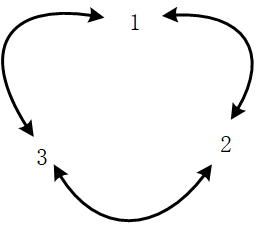
\includegraphics[width=0.5\textwidth]{Figure/指标顺序.png}
	\caption{置换符号的指标顺序}
	\label{fig:指标顺序}
\end{figure}
